% This is samplepaper.tex, a sample chapter demonstrating the
% LLNCS macro package for Springer Computer Science proceedings;
% Version 2.21 of 2022/01/12
%
\documentclass[runningheads]{llncs}
%

%
\usepackage[T1]{fontenc}
\usepackage{comment}
% T1 fonts will be used to generate the final print and online PDFs,
% so please use T1 fonts in your manuscript whenever possible.
% Other font encondings may result in incorrect characters.
%
\usepackage{graphicx}
\usepackage{enumitem}
\usepackage{amssymb}
\usepackage{amsmath}
\usepackage{subcaption}
\usepackage{hyperref}
\usepackage{float}
% Used for displaying a sample figure. If possible, figure files should
% be included in EPS format.
%
% If you use the hyperref package, please uncomment the following two lines
% to display URLs in blue roman font according to Springer's eBook style:
\usepackage{color}
\renewcommand\UrlFont{\color{blue}\rmfamily}
%\urlstyle{rm}
%
\begin{document}
%\bibliographystyle{splncs04}
%\bibliography{LLMs and Data Streams}
%
\title{Large Language Models and Data Streams}
%
%\titlerunning{Abbreviated paper title}
% If the paper title is too long for the running head, you can set
% an abbreviated paper title here
%
\author{Silyu Li}
%
%\authorrunning{F. Author et al.}
% First names are abbreviated in the running head.
% If there are more than two authors, 'et al.' is used.
%
\institute{RWTH Aachen University, Aachen, Germany
%\email{lncs@springer.com}\\
%\url{http://www.springer.com/gp/computer-science/lncs} \and
%ABC Institute, Rupert-Karls-University Heidelberg, Heidelberg, Germany\\
%\email{\{abc,lncs\}@uni-heidelberg.de}
}
%
\maketitle              % typeset the header of the contribution
%
\begin{abstract}
    Large language models, such as ChatGPT, have become widely recognized and are extensively utilized across various domains. However, these models are typically trained on static datasets, lacking updates to new data beyond their initial training set. 
    To enable models that can continuously update themselves based on incoming data, it is necessary to have large language models trained and updated on input data streams.

    In this paper, we begin by outlining the structure and fundamental applications of large language models. Subsequently, we introduce the concept of data streams and provide an overview of current use cases where large language models are adapted to accommodate streaming data. Finally, we summarize the existing challenges associated with integrating large language models with data streams and discuss potential solutions.
\keywords{LLM  \and data streams \and chatGPT.}
\end{abstract}
%
%
%
\section{Introduction}
Large language models have shown their wide usage and significant competence in many fields according to \cite{Liu23}, such as learning and answering users' questions in academic fields,
assisting in diagnosing diseases in medical fields, generating text and classifying text data to various categories and so on. However, as \cite{Gupta23} demonstrates, 
there is a significant limitation of current large language models: they are trained based on certain static datasets that will not automatically be updated, and this causes the resulting models to only be able to access information from its training datasets. 
When the models need to be updated as new data becomes available, the only way is to start the training process over again. But in many scenarios such models can't satisfy our needs. 
For example, to have a better traffic prediction, real-time traffic data is needed \cite{Zhang24},
Analyzing news and events sentiment can help predict the financial market \cite{Araci19}, 
real-time health data is of great importance when monitoring patients' health condition \cite{Thiru23} and so on.
So to have models that can fulfill those use cases, we need to find and compare useful methods that combine large language models and continuous data input (data streams) and also summarize the current major obstacles. 

\section{Related Works}
In this chapter, the following concepts and techniques that are related to this topic will be covered.

\subsection{Large Language Model}
In this subsection, we will first summarize the evolution of language models, followed by an overview of the current large language
models' structure and training process.    
  
\subsubsection{The Evolution of Large Language Models}  
\noindent \newline 
The earliest language models, taking n-grams as an example, are statistical. n-grams refers to an n-words substring of a longer string and n represents the number of words in the substring, according to \cite{Cavnar94}.
Taking the sentence "I read a book" as example, a bi-grams composition of this sentence would be "I read", "read a" and "a book". By considering the n previous words, the frequency and probability of each
n-grams can be calculated, which makes n-grams model perform well in text classification and word prediction with short documents \cite{Cavnar94}. 
However, n-grams performs poorly with long documents due to the rapid growth of dimensionality with large n, and it has only restricted access to the words that appear in the document.\\
\noindent \newline
Later models using word embeddings such as Word2Vec solve the problems of earlier models to some extent by representing words in vector spaces, and words with similar meanings such as "walk" and "run" have closer distance
in the vector space \cite{Mikolov13}. Word embeddings successfully reduces the dimensionality of word representations and can work with larger documents by combining techniques such as "Continuous Bags of Words" \cite{Mikolov13}. \\   
\noindent \newline
With the development of neural networks, more powerful models such as the Seq2Seq model began to take a more important role in many application fields such as
machine translation \cite{Sutskever14}. The core idea of the Seq2Seq model is that it uses the Long Short-Term Memory(LSTM) networks as an encoder to map the input to a vector with fixed dimensionality, and then
uses another LSTM to decode the output sentence from the vector. By regulating the present and past information and gradient flow, LSTM makes it possible for the model to handle long input sequences and the encoder-decoder structure enables the model 
to manage different lengths for input and output sequences \cite{Sutskever14}. \\
\noindent \newline
Large language models start to have a huge leap forward after the introduction of the transformer architecture \cite{Vaswani17}. \cite{Radford18} demonstrates that the transformer architecture can
effectively improve the language understanding ability of language models even with large unlabeled text corpora by first generatively pre-training the model on the text data and then discriminatively fine-tuning them on various tasks.
Modern models usually own a large number of parameters and large-scale training datasets, but the source of the training datasets can vary from model to model. For example, 
according to \cite{Radford19}, GPT-2 (with 1.5 billion parameters) is trained on massive training datasets including the crawling results from millions of different web pages, called WebText. BERT (BERT$_{BASE}$ with 110 million
parameters, BERT$_{LARGE}$ with 340 million parameters) is trained on the English Wikipedia (2,500 million words) and BookCorpus (800 million words), a large dataset of books used for machine learning approaches \cite{Devlin18}. 
A more recent model collection called LLaMA (with 7 to 65 billion parameters) is trained on various open-source data such as commoncrawl\footnote{\url{https://commoncrawl.org/}}, C4, Github, Wikipedia and so on \cite{Touvron23}. 
Table \ref{table:comparison} provides a brief overview of the 3 models together with information on the most recent GPT-3.5 and GPT-4 models according to the OpenAI blog\footnote{https://platform.openai.com/docs/models/gpt-base}. \\

\begin{table}[H]
  \centering
  \begin{tabular}{| p{4cm} | p{2cm} | p{2cm} | p{2cm} | p{2cm} |}
  %\hline
  %\textbf{Aspect} & \textbf{Model 1} & \textbf{Model 2} & \textbf{Model 3} & \textbf{Model 4} \\\textbf{Model Name} & GPT-4 & BERT & T5 & RoBERTa \\
  \hline
  \textbf{Model Name} & BERT & GPT-2 & LLaMA & GPT-3,5/ 4 \\
  \hline
  \textbf{Developer} & GoogleAI & OpenAI & MetaAI & OpenAI \\
  \hline
  \textbf{Release Date} & 2018 & 2019 & 2023 & 2022/2023 \\
  \hline
  \textbf{Nr. of Parameters} & 110 M/ 340 M & 1,5 B & 7-65 B & 175 B/1,7 T \\
  \hline
  \textbf{Training Data} & Wikipedia(en) \& BookCorpus & WebText & Various open-source datasets & WebText \\
  \hline
  \textbf{Open-sourced} & Yes & No & Yes & No \\
  %\hline
  %\textbf{Performance} & SOTA on many NLP tasks & High on NLU tasks & High on text generation and NLU tasks & High on NLU tasks \\
  \hline
  \textbf{Major Applications} & QA & Text generation \& Translation & Text generation \& QA \& Translation & Content generation \& QA \& Translation \\
  %\hline
  %\textbf{Pricing} & Subscription-based & Open-source & Open-source & Open-source \\
  %\hline
  %\textbf{Availability} & API & Downloadable model & Downloadable model & Downloadable model \\
  \hline
  \end{tabular}
  \caption{Comparison of Large Language Models}
  \label{table:comparison}
  \end{table}

\noindent
The parameter size of different models has a growing trend, which can be explained by the relationship between model performance, the number of model parameters $N$, the size of dataset $D$ and the amount of computing to train the model $C$. \cite{Kaplan20} demonstrates the \textbf{Smooth Power Laws} which says:
"Performance has a power-law relationship with each of the three scale factors N, D, C when not bottlenecked by the other two, with trends spanning more than six orders of magnitude". Nowadays, there are various models
that have distinct capabilities, for example, DALL-E can generate and modify images based on text input, whereas ChatGPT 3.5 can generate code and natural language, as \cite{Gozalo23} in figure \ref{fig:model_overview} summaries.
\noindent \newline
\begin{figure}[H]
  \centering
  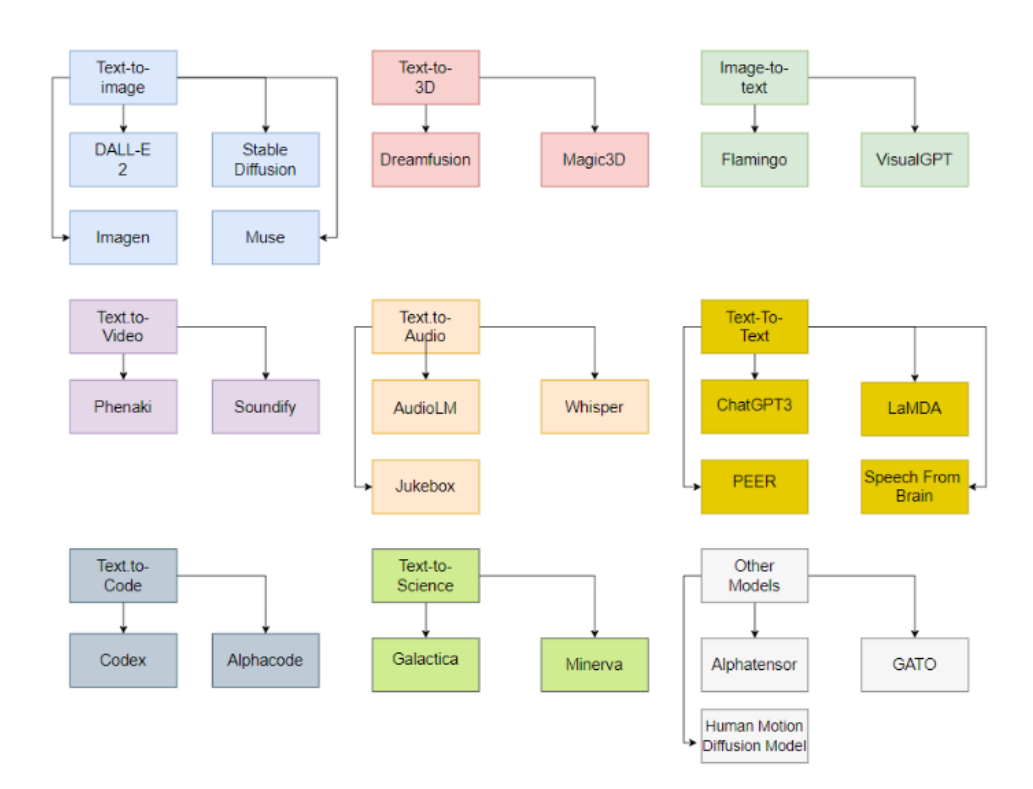
\includegraphics[width=0.8\textwidth]{models overview.png}
  \caption{An overview of the recent major generative AI models  \cite{Gozalo23}}
  \label{fig:model_overview}
\end{figure} 

\subsubsection{The Architecture and Training Process of Large Language Models}
\noindent \newline
Many of the recent large language models such as ChatGPT, LLaMA and BERT are based on transformer-based neural networks. The transformer architecture, as \cite{Vaswani17} in figure \ref{fig:attention} demonstrates, is an 
encoder-decoder architecture. The encoder takes the input sequence and converts them into dense vectors of fixed size at the input embedding step. Then with the 
help of the positional encoding step, the input sequence contains information about each token in the sequence. The encoded inputs are then passed through the multi-head attention mechanism so that the 
model can capture various relationships and features from the input sequence. Then the Add and Normalization layer is applied to stabilize and speed up the training process. In the end, the Feed Forward layer is 
applied to help in introducing non-linearity and learning complex representations for each token's position in the sequence. Similarly, the decoder uses the vector representation of the input sequence created
by the encoder along with the previously generated tokens to produce the next token in the output sequence and the masked multi-head attention mechanism is applied to ensure that the prediction for a particular position depends only on the known outputs at earlier positions. \\

\begin{figure}[H]
  \centering
  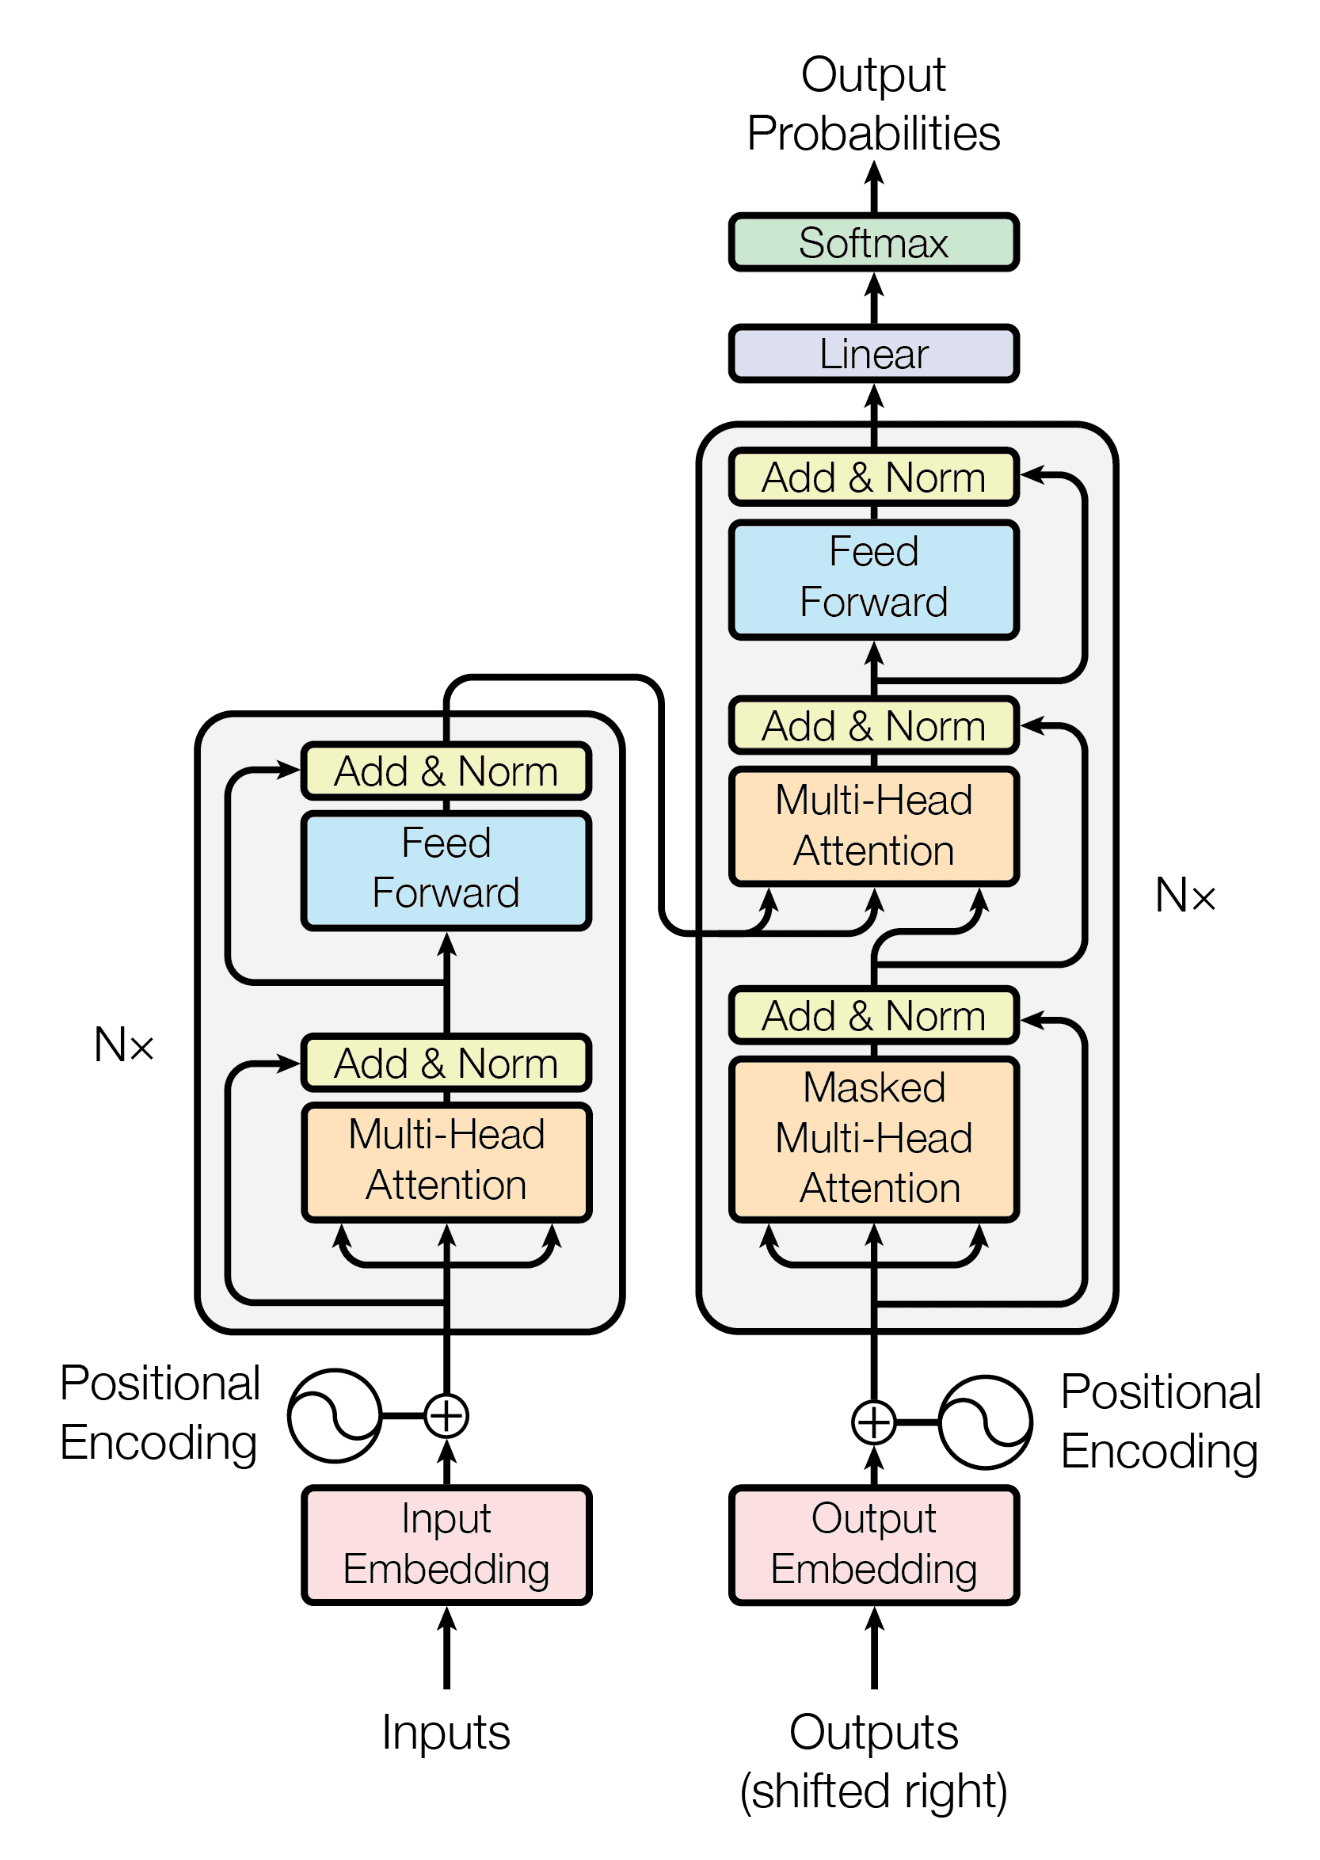
\includegraphics[width=0.6\textwidth]{attention1.jpg}
  \caption{The transformer structure \cite{Vaswani17}}
  \label{fig:attention}
\end{figure}
\noindent \newline
Various input text datasets must be pre-processed as valid input representations before they can be used for the training process, and the data pre-processing includes the following procedures \cite{Roum23}:
\begin{itemize}
  \item Tokenization involves segmenting text into tokens, which are the basic units of broken text. Tokenization can simplify and standardize the input data and improve model performance \cite{Devlin18}.
  \item Subword encoding refers to breaking down the input text into smaller units and helping handle rare or out-of-vocabulary words in the input text.
  \item Data cleaning is the step where the noisy information in the input data should be removed, which can significantly improve the quality and suitability of the input data for the model.
\end{itemize} 
\noindent \newline
More specifically, BERT uses the WordPiece embeddings \cite{Wu16} with a 3000 token vocabulary. For each input, a classification token $([CLS])$ is used to mark the beginning of the sentence and a $([SEP])$ token is
used to mark the end of a sentence. In some cases, several sentences are combined as one single sentence, therefore a new embedding is needed to mark to which sub-sentence each token belongs \cite{Devlin18}.
As figure \ref{fig:bert_input} shows, an example input sentence "My dog is cute, he likes playing." is first tokenized into smaller units, where $([CLS])$ marks the start of the input and 
$([SEP])$ marks the end of the sentence as well as splits the sentence into 2 parts. A token embedding is added for each token, a segment embedding is added to show to which sentence each token belongs and
a position embedding is used to show the position of each token within the sentence. The final input representation is the sum of all embeddings.
\begin{figure}[H]
  \centering
  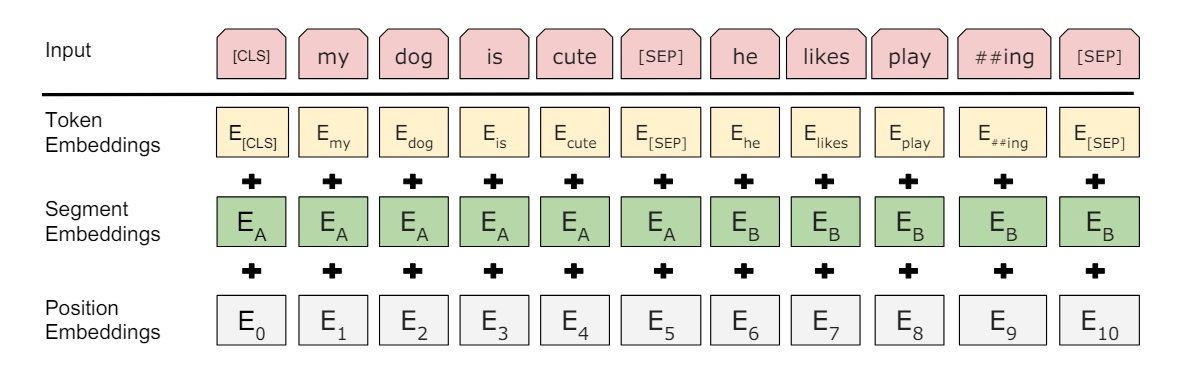
\includegraphics[width=0.8\textwidth]{BERT input repres.png}
  \caption{Input representation of BERT \cite{Devlin18}}
  \label{fig:bert_input}
\end{figure}

\noindent \newline
GPT-2 and LLaMA use Byte Pair Encoding (BPE) \cite{Sennrich15} to tokenize the input text where BPE iteratively count the frequency of the characters or subwords and merge the most frequent ones
to form new vocabulary \cite{Radford19}, \cite{Touvron23}. There are several different implementations of BPE that are moderate for different use cases, the training corpus on which BPE is applied also
significantly influences the size of the result vocabulary. GPT-2 applies BPE with a base vocabulary of more than 130,000 tokens, whereas the BPE applied on LLaMA creates around 1,4T tokens.

\noindent \newline
A model starts its training algorithm after taking the pre-processed data as its input. For recent models such as ChatGPT, LLaMA and BERT, their training algorithms share a same process of an unsupervised pre-training phase and a supervised fine-tuning phase \cite{Roum23}.
In the pre-training phase, a large amount of unlabeled WebText data is used as the model's training dataset to make it a high-capacity language model. Given an unlabeled corpus of tokens $U=\{u_1,...,u_n\}$ as a training dataset, the core idea of the pre-training phase is to 
predict the next token $u_i$ for a sequence $\{u_{i-k},...,u_{i-1}\}$. According to \cite{Radford18}, this is done by maximizing the likelihood: 
\begin{equation}
  L_1(U) = \sum_{i}\log{P(u_i|u_{i-k},...,u_{i-1}; \Theta)}
\end{equation}
$k$ refers to the context window size and $\Theta$ is the parameter of the neural network with which the conditional probability $P$ is modeled. \\
\noindent \newline
The supervised fine-tuning phase is used to improve the model's performance on specific tasks by training it on a smaller corpus of labeled data \cite{Roum23}. Given a labeled dataset $C$,
where each instance of $C$ has a sequence of tokens \{$c^1,...,c^m$\} and a label $y$, the goal of the fine-tuning phase is to maximize the following likelihood \cite{Radford18}:
\begin{equation}
  L_2(U) = \sum_{(x,y)}\log{P(y|x^1,...,x^m)}
\end{equation}

\noindent \newline
In the BERT model, as shown in figure \ref{fig:bert_finetune}, the pre-training phase consists of 2 unsupervised tasks: Masked LM and Next Sentence Prediction (NSP).
Masked LM is used to help BERT understand the context of words within a sentence, it masks 15\% of all WordPiece tokens in each input sentence and the model 
predicts only the masked words instead of reconstructing the entire input. NSP is applied to help BERT understand the relationship between 2 sentences. More specifically, when 
having 2 sentences A and B as input, B is replaced by another random sentence from the training set for half of the time and remains unchanged for the other half of the time.
The BERT is trained to predict whether the second sentence in the input is the actual sentence B. According to \cite{Devlin18}, NSP has significant benefits for question answering (QA).
Fine-tuning BERT is relatively inexpensive compared with pre-training, as it only involves fine-tuning the parameters while feeding BERT with various task-specific inputs and outputs 
such as QA tasks, single sentence classification tasks, sentence pair classification tasks and so on. When fine-tuning, an additional output layer is added to BERT so that the minimal number of 
parameters need to be learned from scratch again.

\begin{figure}[H]
  \centering
  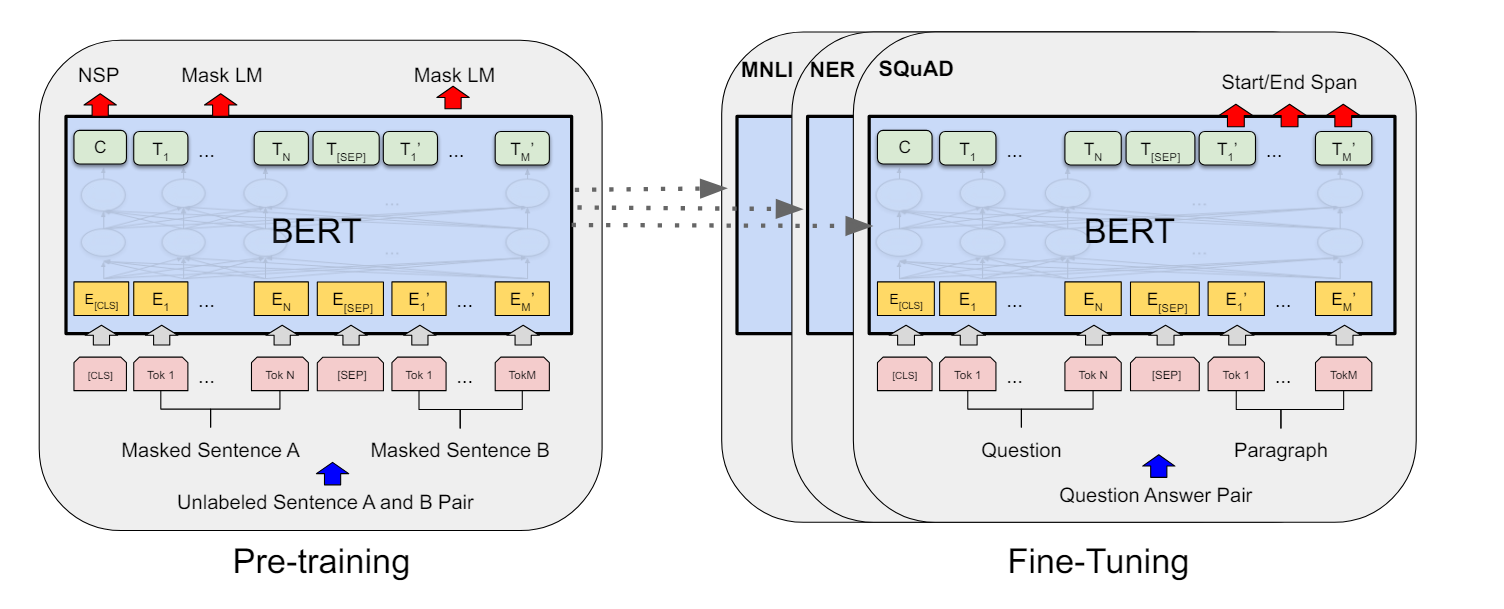
\includegraphics[width=0.95\textwidth]{BERT Finetuning.png}
  \caption{Training process in the BERT model \cite{Devlin18}}
  \label{fig:bert_finetune}
\end{figure}

\noindent \newline
GPT-2 and LLaMA make some improvements to the pre-training process such as normalizing the input for each transformer layer and adding a normalization layer
after the last self-attention layer to improve the training stability (GPT-2 and LLaMA) \cite{Radford19}, replacing the ReLU layer with a SwiGLU layer to improve model performance (LLaMA) and
replacing the absolute positional encoding with the rotary positional embeddings (RoPE) to increase efficiency and scalability (LLaMA) \cite{Touvron23}. Together with more efficient code implementation
GPT-2 and LLaMA gain better scores on many evaluation fields such as QA, reading comprehension, summarization, translation and so on. Similarly, GPT-2 and LLaMA are fine-tuned with various tasks,
figure \ref{fig:gpt_finetune} illustrates some fine-tuning tasks of the original GPT.



\begin{figure}[H]
    \centering
    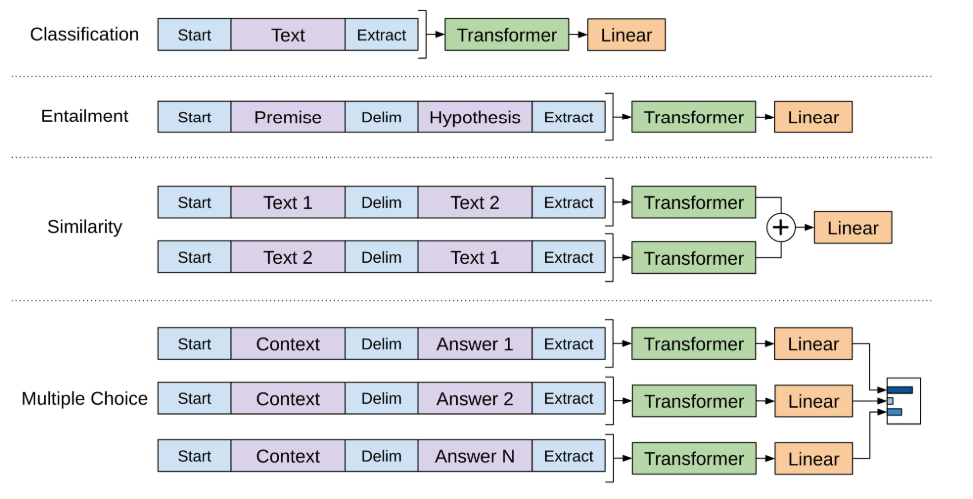
\includegraphics[width=0.8\textwidth]{gpt finetune.png}
    \caption{Fine-tuning of GPT \cite{Radford18}}
    \label{fig:gpt_finetune}
\end{figure}

\subsection{Data Stream}
In many application fields nowadays, data is often generated and processed at a very high rate. These include health sensors that track body temperature and blood pressure \cite{Geisler13},
monitoring of production lines, information on stock trading, posted content on social networks and so on. \cite{Geisler16}. Due to its near real-time and huge amounts characteristics, traditional data management
approaches are often not suitable anymore, a new system called Data Stream Management Systems (DSMS) which supports continuous queries, low latency processing, simple scalability and resource management
 has evolved to address this issue \cite{Geisler16}. \\
\noindent \newline
Data stream has many informal definitions, \cite{Patro06} describes data stream as "time-varying, volatile, unpredicted and possibly unbounded information". \cite{Golab03} describes data stream as
"a data set that is produced incrementally over time, rather than being available in full before its processing begins". According to \cite{Geisler13}, a data stream has the following formal definition:
\begin{definition}
  A data stream $S$ is an unbounded, potentially infinite multiset of data stream elements $(s,\tau)$, where $\tau \in \mathbb{T}$. $\mathbb{T}$ is a timestamp attribute with values from a monotonic, infinite time domain $\mathbb{T}$ with discrete time units.
\end{definition} 
\noindent
There are multiple methods to analyze data streams, \cite{Gaber05} categorizes them into data-based and task-based solutions. Data-based solution refers to examining a subset of the data stream and approximating to an
overall outcome for the data stream. Task-based solutions, on the other hand, often refer to achieving time and space efficiency in computing by using relevant techniques. We summarize some of the solutions:
\begin{itemize}
  \item Synopsis is a data-based solution and it refers to the process of creating compact data summaries such as wavelet analysis and histograms, which can efficiently approximate and query large data streams without processing the entire dataset \cite{Gaber05}.
  \item Window is a task-based solution and it refers to adjusting a continuous data stream into bounded segments of data (windows), each window is executed over the items of a single data stream and returns a concrete and finite data segment \cite{Patro06}.
\end{itemize}

\section{LLMs with Data Streams}
Although large language models have shown strong capabilities in many application fields, their knowledge remains static as they are pre-trained on static datasets. In some occasions, however, a user query
expects up-to-date results. Considering the following questions: \textit{Who is the current president of the USA?} The answer to such a question expires likely every 4 years, which seems a reasonable time
for an update of the large language model's training datasets. The question \textit{What are the results of the last Bundesliga match day?} would require the knowledge of large language models to be updated
at least every week. The question \textit{What is the current traffic condition in the Königstraße of city Aachen?} would require even a near real-time result. Thus, in many application fields, the performance of a 
pre-trained large language model is likely to gradually degrade over time \cite{Shi24}. In this section, we will first summarize some approaches where large language models are combined with data streams, then discuss some common issues and challenges in this field.
Finally, we will list some use cases that address some of the challenges.

\subsection{Continual Learning}
The need for regular updates of large language models brings intense focus to the concept of \textbf{Continual Learning}.  

\subsubsection{Continual Learning of LLMs} 
\noindent \newline
According to \cite{Biesi20}, continual learning refers to the process of accumulating knowledge on non-stationary data. In the context of large language models, continual learning is applied to enable LLM models
to learn from a continuous data stream over time. For a data stream of tasks $\mathcal{T}= \{\mathcal{T}_1,\ldots,\mathcal{T}_n \}$, the goal is to
have the model learn sequentially based on the input stream, where it only has access to $\mathcal{T}_i$ at time $i$. \cite{Wu24}, in their continual learning framework for large language models, categorizes 
continual learning into 3 stages as figure \ref{fig:acl_stages} shows:
\begin{itemize}
  \item \textbf{Continual Pre-training (CPT)}: It refers to incrementally updating a large language model on input data over time without retraining it from scratch. It can be further categorized into 
  \textit{CPT for updating facts} which adapts a model to new factual knowledge, \textit{CPT for updating domains} that enriches a model's knowledge in specific fields and \textit{CPT for language expansion} which helps a model
  support more languages.
  \item \textbf{Continual Instruction Tuning (CIT)}: It refers to continuously refining the model's ability to follow the instruction. It can be further categorized into \textit{Task-Incremental CIT} for finetuning a model on a series 
  of tasks to be capable of solving new tasks, \textit{Domain-incremental CIT} for finetuning a model on some continuous instructions so that it can solve domain-specific problems and \textit{Tool-incremental CIT} for 
  continually advising a model to use new tools for problem-solving.
  \item \textbf{Continual Alignment (CA)}: It refers to adjusting the model so it always produces output that satisfies certain standards and guidelines. This can be categorized into \textit{Continual Value Alignment} that continually
  align a model with current ethical and social guidelines and \textit{Continual Preference Alignment} that dynamically adapt a model to different user preferences.
\end{itemize}
\begin{figure}[H]
  \centering
  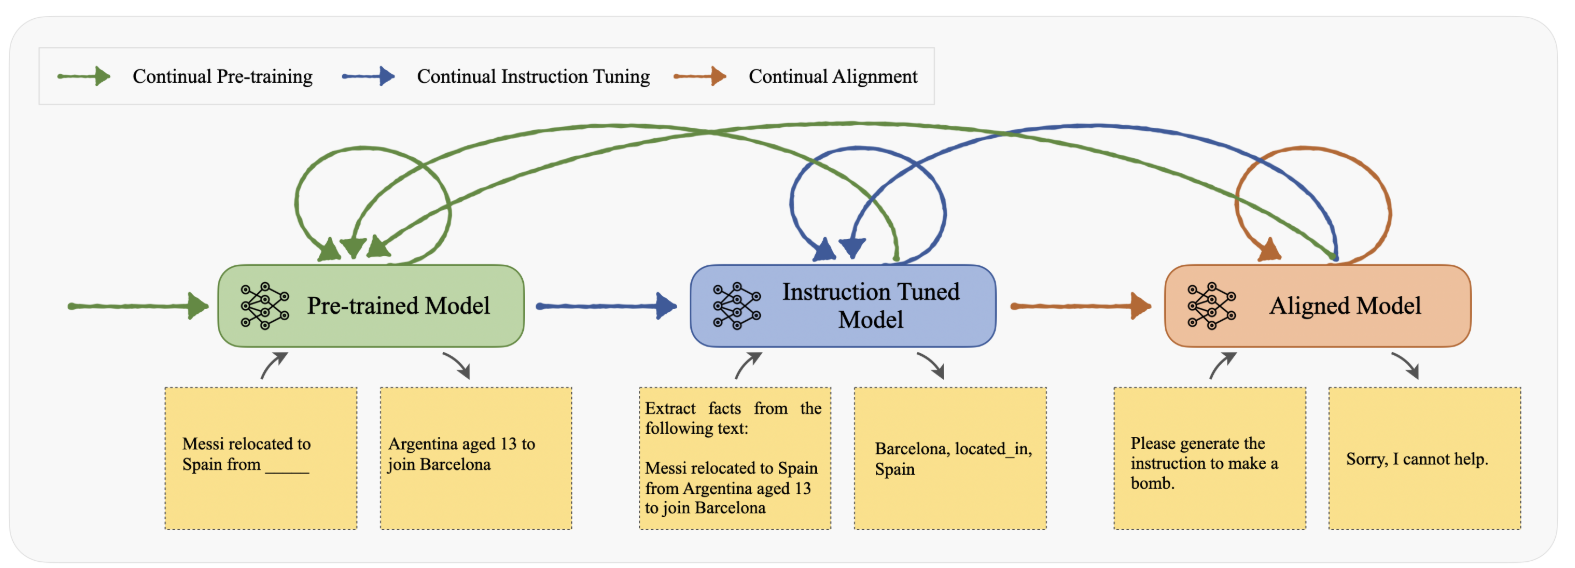
\includegraphics[width=0.95\textwidth]{CL stages.png}
  \caption{Stages of continual learning \cite{Wu24}}
  \label{fig:acl_stages}
\end{figure} 

\subsubsection{Challenge of CL}
\noindent \newline
A critical challenge of continual learning is catastrophic forgetting, which refers to the models forgetting previously learned knowledge 
when they are updated with new data \cite{Gupta23}. Catastrophic forgetting happens in the continual pre-training stage as the model is continuously updated with a data stream.
\cite{Shi24} demonstrates that there are various methods of computing continual learning while mitigating
catastrophic forgetting \cite{Gupta23} and categorizes them as follows:
\begin{itemize}
  \item Replay-Based Methods: The model keeps a small subset of previous tasks and re-trains them periodically.
  \item Regularization-Based Methods: The capacity of the model is typically fixed, and the model adds a regularization term (typically a loss function)
that reflects the consolidation of previous knowledge.
  \item Architecture-Based Methods: Change the architecture of the model for each new task and introduce new parameters that fit the task.
\end{itemize}
\noindent \newline
The architecture-based methods often face the problem of the growing 
training cost, as their models' parameter size grows with new tasks linearly\cite{Jovanov}. The regularization methods avoid the expanding parameters challenge but the computational cost
increases due to the extra computation of the regularization term \cite{Wang24}. Therefore, the replay-based methods are often considered to be
a better approach considering large data stream input, although the choice of selecting the right exemplars from previous tasks can still be difficult \cite{Jovanov}. \\
\noindent \newline
Another challenge of continual learning is concept drift, where the relationship and distribution of input data change over time \cite{Biesi20}. Concept drift often causes the large language models' performance to decrease
due to the discrepancies between the models' output based on previous data and current factual accuracies, societal norms and standards. Therefore the continual alignment stage of continual learning is essential to 
mitigate the effect of concept drift, as it continuously refines the model to align with the current standard \cite{Taori23}.
However, to ensure the right alignment of the model, huge computational resources and human oversight are often required. Additionally, aligning a model to changes without introducing new bias and the protection of data
privacy and security are also challenges to the continuous alignment stage \cite{Shi24}. \\
\noindent \newline
Furthermore, recent studies also point out some other challenges that continual learning with LLM is currently facing \cite{Yang24}.
\begin{itemize}
  \item \textbf{Lack of real-world assumption}. In the training process of an LLM, different datasets are usually merged to create new training datasets. However, this often leads to results that
  lack diversity and real-world complexity. Simple tasks such as text classification and sentiment analysis all have clear labels, but in the real-world assumption, many labels are not always available 
  due to noise. This may reduce the robustness of an LLM.  
  \item \textbf{Multi-modal Continual Learning}. Current continual learning approaches mainly focus on the field of NLP tasks such as sentiment analysis and text classification, but multimodal tasks such aspects
  text-to-image retrieval, text-image classification, and visual question answering would be some possible future work directions of CL. However, this would require the integration of multi-modal datasets with various data types,
  which can be costly and complex. 
\end{itemize} 


\subsubsection{Use Cases}
\noindent \newline
Continual learning is already applied in the field of linguistics, one example is from \cite{Fujii24}, where they discovered the fact that some large language models are trained on English datasets and their performance 
in other languages differs from their performance in English. They came up with the idea of developing a large language model that has strong performance in Japanese and decided to apply continual learning methods, especially 
the continual pre-training stage, on an English LLM LLaMA 2 due to the high computational cost of training an LLM in Japanese from scratch. The idea was to apply continual learning so that the LLaMA 2 model could adapt its knowledge 
and capabilities to Japanese and to construct a model called Swallow in the end. \\
\noindent \newline
According to \cite{Fujii24}, Swallow preserves the same architecture as LLaMA 2, such as its number of attention heads and its number of layers. To prevent catastrophic forgetting, they applied the replay-based method
by selecting 5\% of the training data from English RefinedWeb \cite{Penedo23}, 5\% from the English arXiv paper texts and the remaining 90\% from Japanese texts. After developing Swallow, they evaluate its performance in various fields such
as question answering (QA), reading comprehension (RC), automatic summarization (AS), arithmetic reasoning (AR), commonsense reasoning (CR) and machine translation(MT) and compare its performance to the original LLaMA 2 model.
The results showed that despite the large data stream input, Swallow managed to have a better performance in many fields compared with LLaMA 2, especially in QA task as figure \ref{fig:swallow} shows.
\begin{figure}[H]
  \centering
  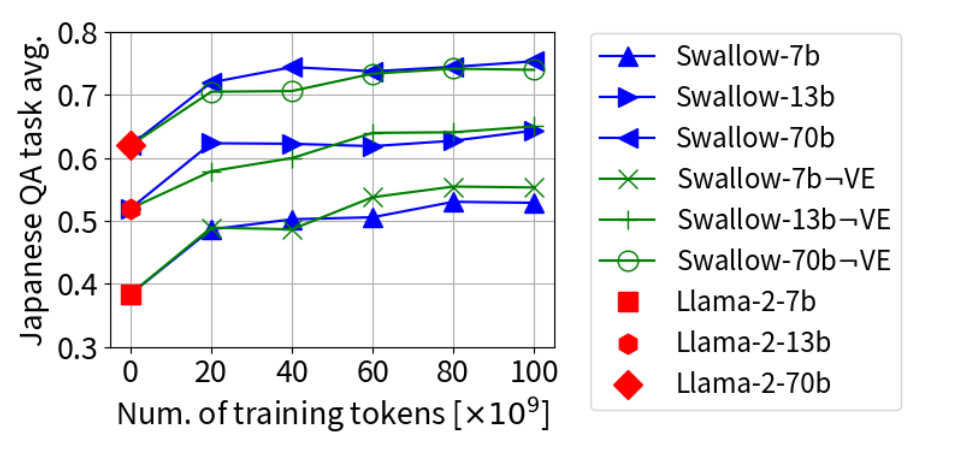
\includegraphics[width=0.8\textwidth]{swallow.png}
  \caption{Performance curve of the Swallow model in question answering task \cite{Fujii24}}
  \label{fig:swallow}
\end{figure}

\noindent \newline
A more recent study proposes another technique called \textit{Progressive Prompt} based on continual learning, while typical continual learning methods train a model on various large datasets, progressive prompt only needs
to learn less than 0,1\% of all parameters but still match the performance of continual pre-training and fine-tuning on large datasets \cite{Razda23}. Before Progressive Prompt is proposed, another technique called \textit{Progressive Network}
was proposed to help a model continually learn from new tasks without catastrophic forgetting \cite{Rusu16}. The idea of Progressive Network is to freeze the network of parameters learned from a previously task prompt and let it stay accessible by copying it to new
network of incoming tasks. Since the learned parameters are frozen while learning new networks, it can mitigate the effect of catastrophic forgetting. However, Progressive Network adds a new copy of the model for each task, causing it extremely 
computationally expensive for large language models with more parameter size, as figure \ref{fig:progressive} shows. In Progressive Prompt, however, a separate prompt is learned for each new task and is sequentially concatenated from learned prompts.
That means the frozen parameters are not copied, but directly accessible to the parameters of new task prompts. Progressive Prompt shows significant improvement in efficiency and can be applied to all transformer-based architecture.
\begin{figure}[H]
  \centering
  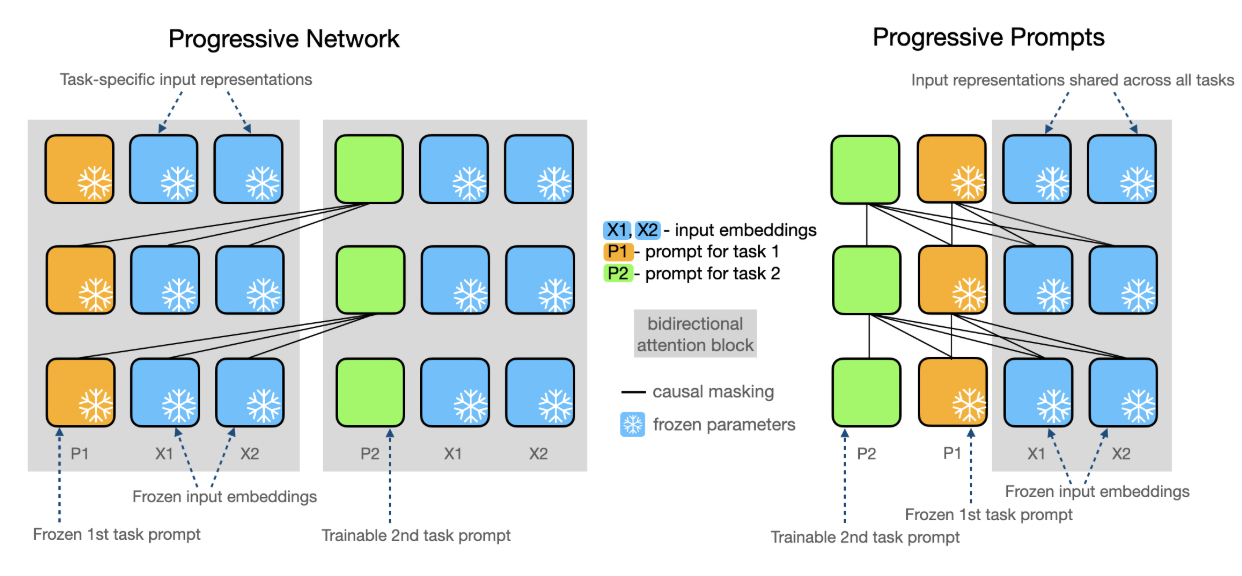
\includegraphics[width=0.9\textwidth]{progressive.png}
  \caption{Illustration of Progressive Network and Progressive Prompt \cite{Razda23}}
  \label{fig:progressive}
\end{figure}

\subsection{Prompt Engineering}
\subsubsection{Definition}
\noindent \newline
\cite{LiuPengfei23} defines a prompt as "a set of instructions provided to an LLM that programs the LLM by customizing it and/or enhancing or refining its capabilities" and prompt engineering
as "the means by which LLMs are programmed via prompts". More specifically, Prompt engineering is the process of providing large language models with effective inputs or queries to elicit specific, high-quality responses \cite{Zhang24}.
It has been proven to have a positive influence on the performance of many downstream tasks such as text summarization, sentiment analysis,
and natural language translation \cite{Liu21}. Considering the following prompt:
\begin{example}
  "Write a detailed and engaging introduction for a blog post about the benefits of learning Python for data science. Highlight at least three key advantages and provide real-world examples to illustrate each point."
\end{example}
By giving the prompt, the large language model is required to give an engaging, detailed and structured answer to the topic of the benefits of learning Python for data science.
Figure \ref{fig:both_prompts} shows an example of how different prompts guide ChatGPT to provide different outputs over the same topic.
\begin{figure}[H]
  \centering
  \begin{subfigure}[b]{0.48\textwidth}
      \centering
      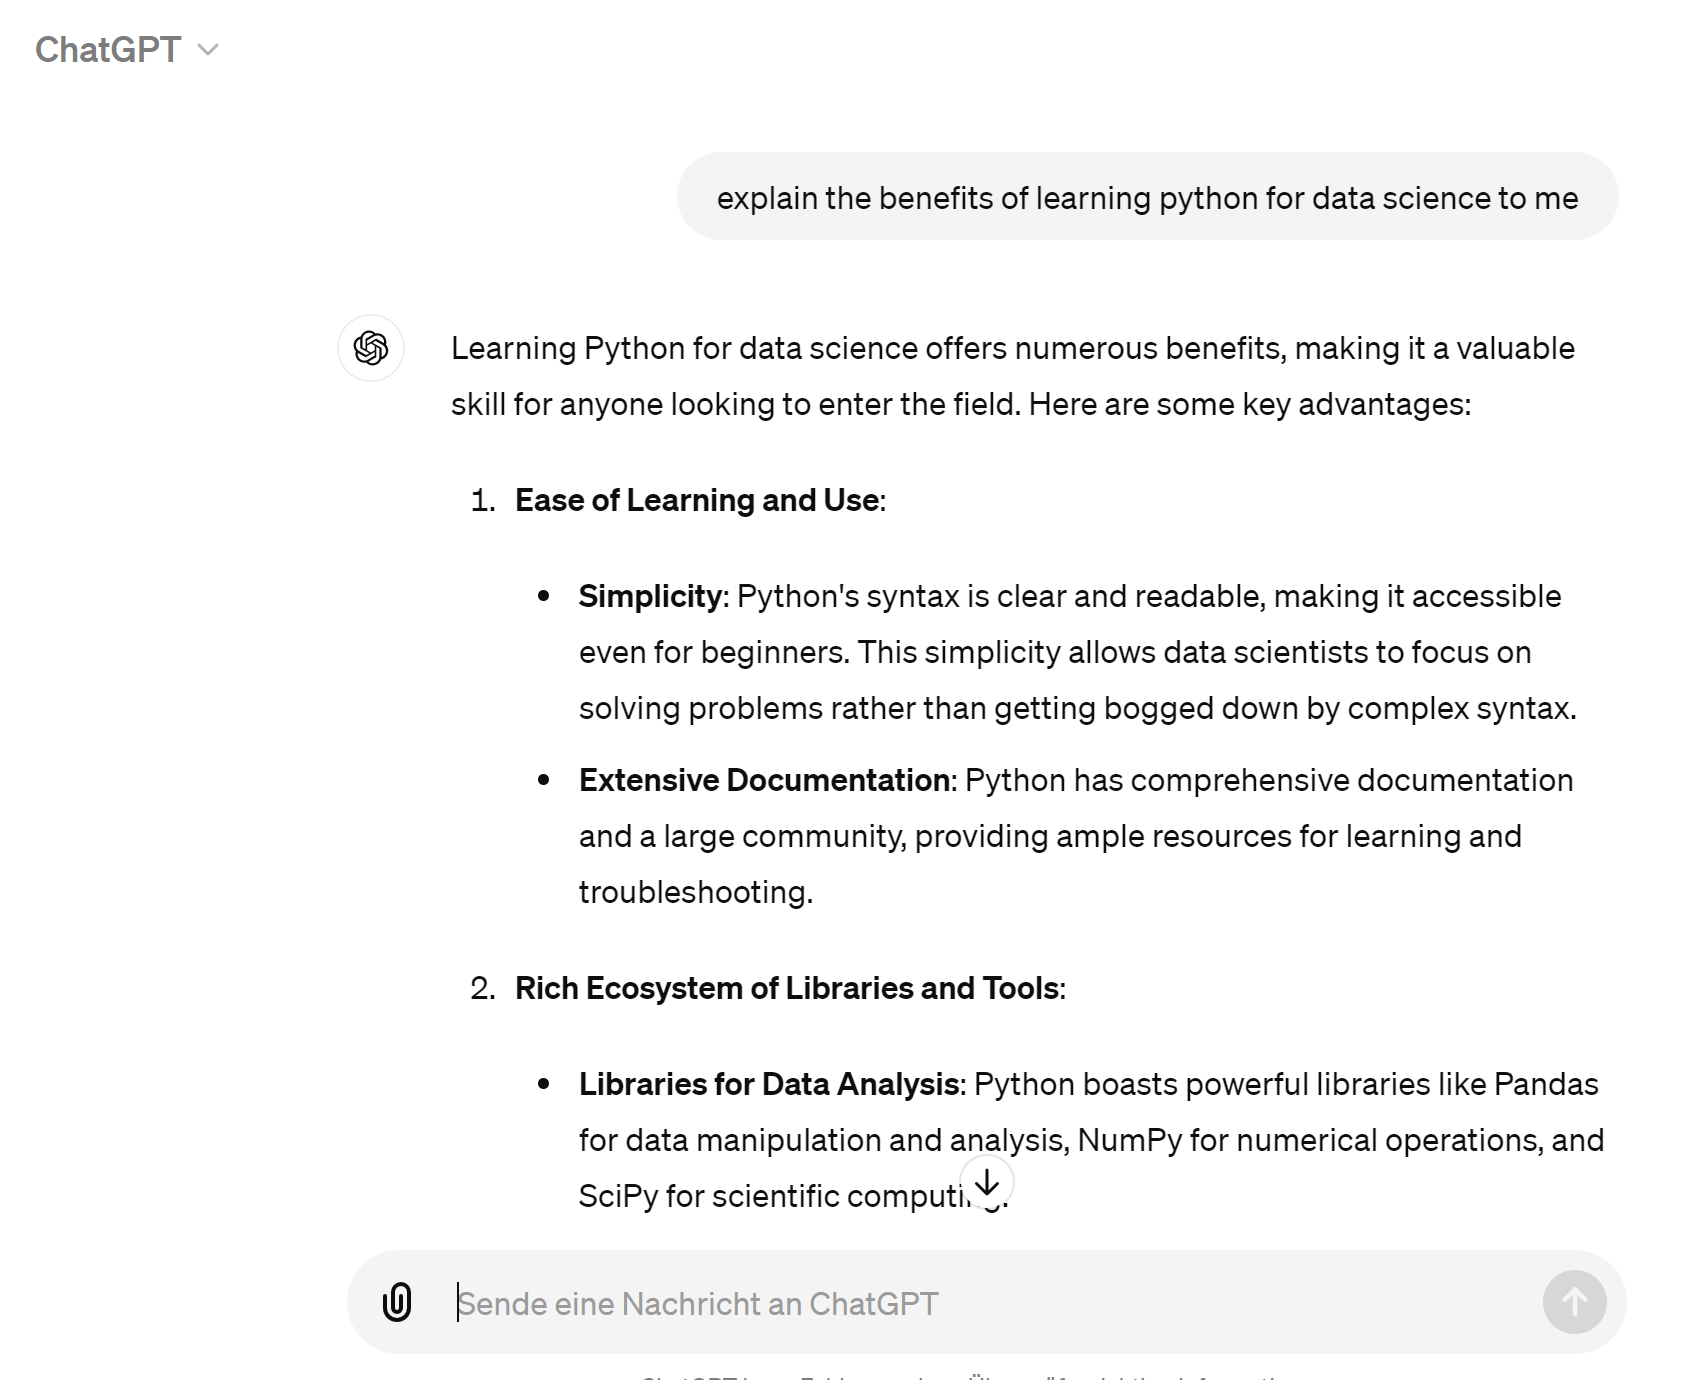
\includegraphics[width=\textwidth]{prompt_ds_1.PNG}
      \caption{Prompt 1}
      \label{fig:prompt1}
  \end{subfigure}
  \hfill
  \begin{subfigure}[b]{0.48\textwidth}
      \centering
      
\includegraphics[width=\textwidth]{prompt_ds_2.PNG}
      \caption{Prompt 2}
      \label{fig:prompt2}
  \end{subfigure}
  \caption{2 different prompts yield different output of ChatGPT}
  \label{fig:both_prompts}
\end{figure}

\subsubsection{Challenges}
\noindent \newline
\cite{White23} demonstrates the quality of the prompt provided by users as the major factor that affects the output quality of large language models using prompt engineering
Furthermore, they demonstrate that prompt formulation should follow the specific prompt pattern and summarize the components of a prompt pattern as follows:
\begin{itemize}
  \item A name and classification: It uniquely identifies the prompt pattern and indicates the issue being addressed.
  \item The intent and context: It describes the issue.
  \item The motivation: It explains the importance of this issue.
  \item The structure and key ideas: They provide the LLM with important contextual information.
  \item Example implementation: It provides an example prompt pattern that can be referenced for other pattern formulations.
  \item Consequences: It explains the possible effect of this prompt pattern.
\end{itemize}
However, \cite{White23} also points out that for different issue categories such as "Alternative Approaches Pattern" (which guides the model to output alternative options) and "Fact Check List Pattern" 
(which guides the model to provide a list of facts), the specific implementation of each component could differ. \\

\noindent \newline
To enhance prompt engineering and evaluate the output of large language models, \cite{Arawjo24} proposes a tool called \textbf{ChainForge}. The core idea is to provide a user interface so that users
can first select and adjust the prompt template, select the LLM models to be evaluated and see the evaluation of the responses from the selected models. The system provides users with high-level
flexibilities such that users can define their evaluation rules using an evaluator in the system, select multiple models to have an overview of their performance according to the evaluation rules
and send multiple requests easily by chaining prompt templates. Figure \ref{fig:chainforge} shows the workflow of ChainForge where 2 different prompt templates are chained using the same input variable in \{\} brackets.
By chaining the 5 input elements with the \{game\} variable, the system can send 10 requests at once to each LLM model selected. With the help of ChainForge, users can evaluate the quality of a prompt on various models more easily. 

\begin{figure}[H]
  \centering
  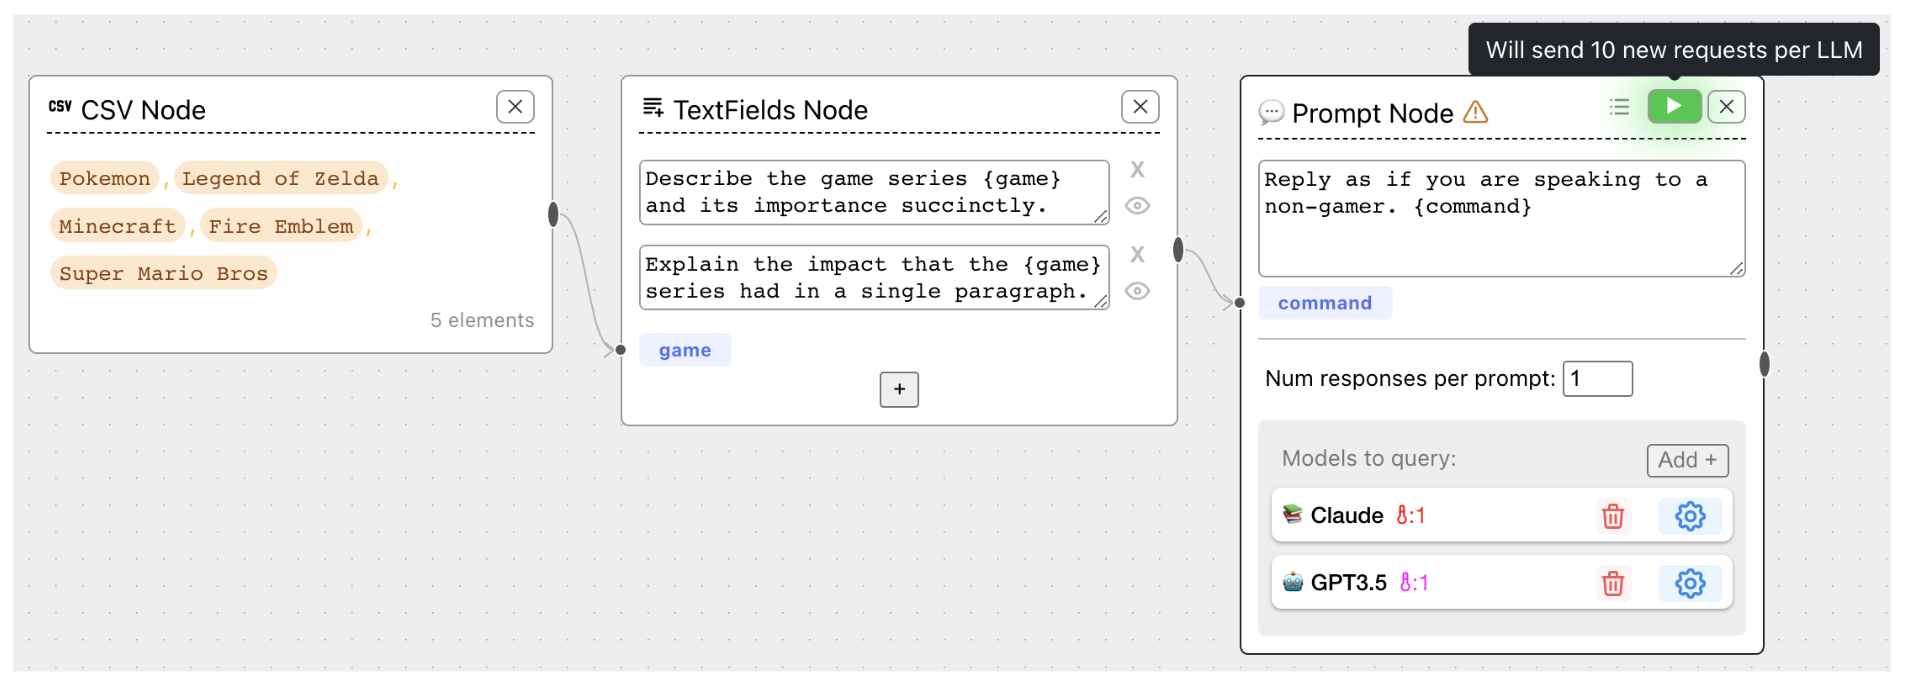
\includegraphics[width=0.95\textwidth]{chainforge.png}
  \caption{The workflow of ChainForge \cite{Arawjo24}}
  \label{fig:chainforge}
\end{figure}

\subsubsection{Use Cases}
\noindent \newline
In the field of traffic signal control, \cite{Lai23} proposes a model called LLMLight based on large language models to act as a decision-making agent. As figure \ref{fig:llmlight} shows,
An LLMLight agent is responsible for controlling the traffic light at an intersection. Real-time observations about the traffic condition are converted into human-readable text and transferred to 
the model, followed by the prompt engineering formed by the real-time observations, task descriptions and control action.
\begin{figure}[H]
  \centering
  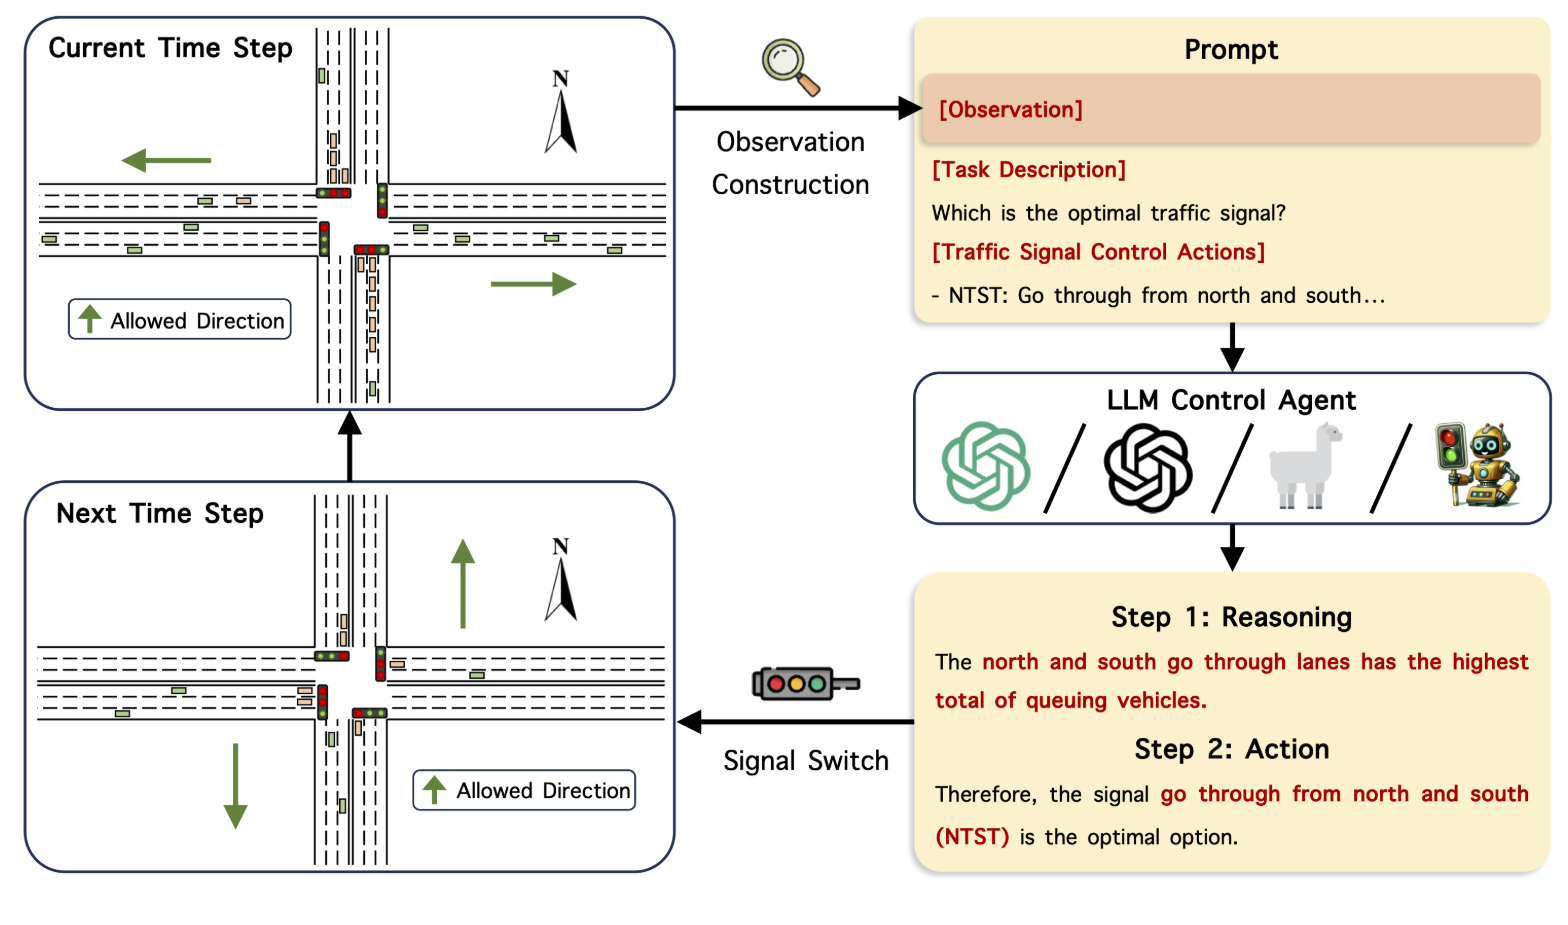
\includegraphics[width=0.95\textwidth]{LLMLight.PNG}
  \caption{The workflow of LLMLight \cite{Lai23}}
  \label{fig:llmlight}
\end{figure}
\noindent
\cite{Lai23} also formulates the workflow as the following equation:
\begin{definition}
  $(Y, a) = \pi_{\theta}(\text{Prompt}(o, d_{\text{scene}}, d_{\text{task}}, d_{\text{know}}, A))$.
\end{definition}
Where $\pi_{\theta}$ refers to the traffic signal control policy, $(Y, a)$ refers to the reasoning trajectory and the action output by the model,
based on the real-time traffic condition observation $o$, traffic scenario description $d_{\text{scene}}$, task descriptions $d_{\text{task}}$ , commonsense knowledge $d_{\text{know}}$, and control action space $A$.
Figure \ref{fig:llmlight_prompt} shows an example template of the prompt \cite{Lai23}.

\begin{figure}[H]
  \centering
  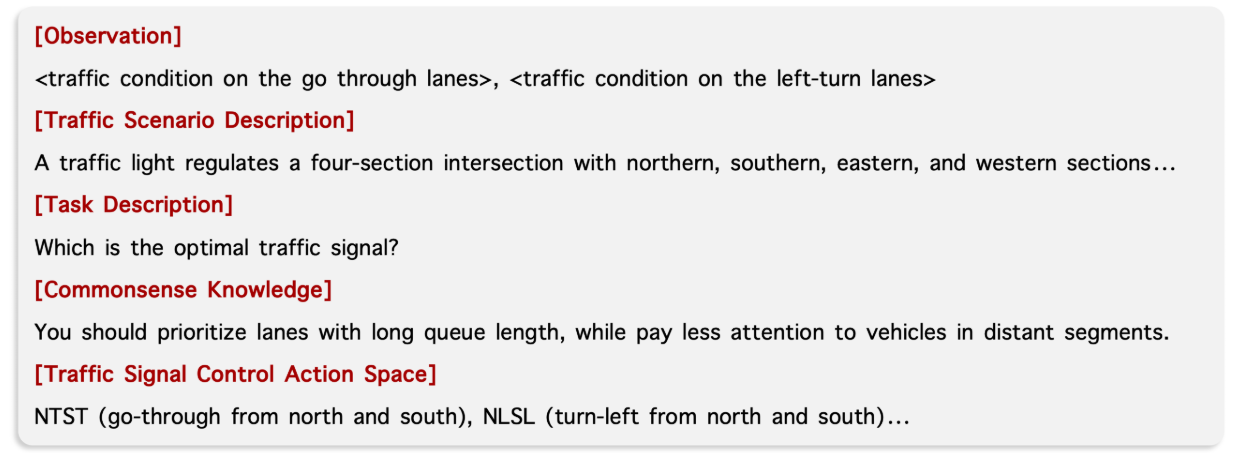
\includegraphics[width=0.95\textwidth]{Prompt LLMLight.PNG}
  \caption{Prompt template \cite{Lai23}}
  \label{fig:llmlight_prompt}
\end{figure} 
\noindent 
Prompt engineering is also applied in the field of traffic data imputation, \cite{Zhang24} proposes a Graph Transformer-based Traffic Data Imputation (GT-TDI) model to compute the missing and faulty values from 
the large-scale road network traffic data streams collected by various sensors, both road-attached and vehicle-carried. The core idea of the GT-TDI model is to model sensors and their relations as nodes and edges in 
a road network graph, the graph is later processed by a Graph Neural Network component. The data streams collected by sensors are transformed into many prompts with a series of semantic descriptions that contain the spatiotemporal information of the network,
they are then encoded and passed to the GT-TDI model. By training on the input datasets, the model is then fine-tuned in the domain of traffic data. Finally, by providing the correct prompt such as 
\textit{"Predict the missing traffic volume for sensor B456 between 3 PM and 4 PM considering the last known values and nearby sensors' data."}, the corresponding missing value can be computed by the model based on the similarity of historical training data
and the input prompt, As figure \ref{fig:TStreamLLM} illustrates. 

\begin{figure}[H]
  \centering
  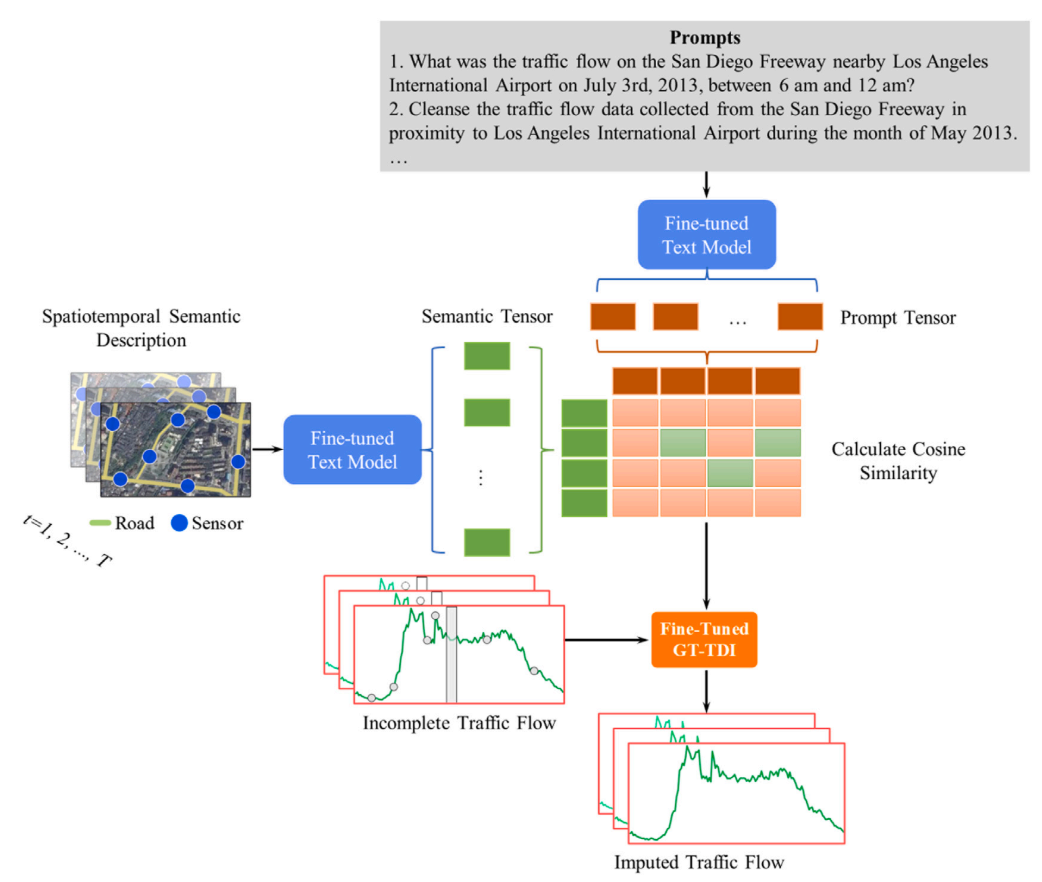
\includegraphics[width=0.5\textwidth]{GT-TDI.png}
  \caption{Implementation of GT-TDI with prompts \cite{Zhang24}}
  \label{fig:TStreamLLM}
\end{figure}

%\section{Conclusion}
%This paper discussed the gap between large language models, which are pre-trained on massive static datasets,
%and data streams, which are continuous and potentially unbounded. Two approaches were presented to mitigate this issue. 
%The first approach, continual learning of large language models, enables the model to continually pre-train over data stream input.
%By applying continual instruction tuning and continual alignment, the model can adapt to the continuous data input. However,
% catastrophic forgetting is likely to occur during this process, so replay-based, regularization-based,
%  and architecture-based methods are applied to mitigate its effects. The second approach, applicable in some fields,
%   involves converting the data stream input into model-readable input and updating the model's knowledge via prompt engineering.
%    This method, however, heavily relies on the quality of the prompts formulated by users.

\section{Conclusion}
This paper addressed the gap between large language models, which are pre-trained on massive static datasets, and data streams, which are continuous and potentially unbounded.
Two main approaches were summarized to mitigate this issue. 
The first approach involves the continual learning of large language models, allowing them to pre-train continually over data stream inputs. 
By applying continual pre-training, continual instruction tuning and continual alignment, the model can adapt to continuous data inputs.
However, catastrophic forgetting is likely to occur during this process, so replay-based, regularization-based, and architecture-based methods are applied to mitigate its effects. 
The second approach converts data stream input into model-readable inputs and updates the model's knowledge via prompt engineering, which relies heavily on the quality of the prompts formulated by users. \\
\noindent \newline
However, there are several shortcomings in this analysis. Firstly, since several models such as ChatGPT and GPT4 are not open-sourced, their exact training process and architecture details remain unknown, 
making it hard to draw a detailed comparison between different models. Secondly, although the two approaches are presented, their real-world applications are still very limited. Powerful large language models  
were mostly developed and applied in recent years, and the usage of LLMs with data streams makes this an even newer topic. Lastly, the assumption that models always have access to regular data for their algorithms is problematic. 
In reality, data is often irregular and multi-modal, making it costly to transform into a usable format. \\
%while promising, still faces challenges related to catastrophic forgetting and the computational overhead associated with continual retraining. 
%Secondly, the reliance on high-quality prompts in the second approach poses a limitation, as it requires significant human effort and expertise to formulate effective prompts consistently.
\noindent \newline
Therefore in future work, 
developing more efficient algorithms to reduce the computational overhead of CA while mitigating catastrophic forgetting is essential. 
For prompt engineering, automating the prompt generation process and improving the model's ability to understand and generate effective prompts autonomously could enhance its applicability. 
Additionally, exploring more real-world application fields is essential for gaining a comprehensive understanding of LLMs with data streams.

%In conclusion, while this paper makes significant strides in adapting large language models to continuous data streams, 
%further research and development are needed to overcome existing challenges and fully realize the potential of these approaches.


%\paragraph{Sample Heading (Fourth Level)}
%The contribution should contain no more than four levels of
%headings. Table~\ref{tab1} gives a summary of all heading levels.
\begin{comment}
\begin{table}
\caption{Table captions should be placed above the
tables.}\label{tab1}
\begin{tabular}{|l|l|l|}
\hline
Heading level &  Example & Font size and style\\
\hline
Title (centered) &  {\Large\bfseries Lecture Notes} & 14 point, bold\\
1st-level heading &  {\large\bfseries 1 Introduction} & 12 point, bold\\
2nd-level heading & {\bfseries 2.1 Printing Area} & 10 point, bold\\
3rd-level heading & {\bfseries Run-in Heading in Bold.} Text follows & 10 point, bold\\
4th-level heading & {\itshape Lowest Level Heading.} Text follows & 10 point, italic\\
\hline
\end{tabular}
\end{table}


\noindent Displayed equations are centered and set on a separate
line.
\begin{equation}
x + y = z
\end{equation}
Please try to avoid rasterized images for line-art diagrams and
schemas. Whenever possible, use vector graphics instead (see
Fig.~\ref{fig1}).

\begin{figure}
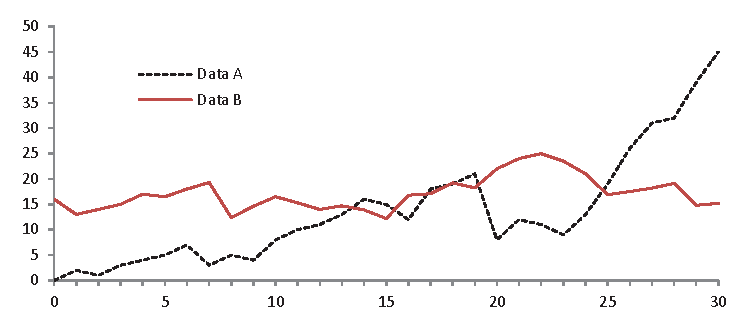
\includegraphics[width=\textwidth]{fig1.eps}
\caption{A figure caption is always placed below the illustration.
Please note that short captions are centered, while long ones are
justified by the macro package automatically.} \label{fig1}
\end{figure}

\begin{theorem}
This is a sample theorem. The run-in heading is set in bold, while
the following text appears in italics. Definitions, lemmas,
propositions, and corollaries are styled the same way.
\end{theorem}
%
% the environments 'definition', 'lemma', 'proposition', 'corollary',
% 'remark', and 'example' are defined in the LLNCS documentclass as well.
%
\begin{proof}
Proofs, examples, and remarks have the initial word in italics,
while the following text appears in normal font.
\end{proof}
For citations of references, we prefer the use of square brackets
and consecutive numbers. Citations using labels or the author/year
convention are also acceptable. The following bibliography provides
a sample reference list with entries for journal
articles~\cite{ref_article1}, an LNCS chapter~\cite{ref_lncs1}, a
book~\cite{ref_book1}, proceedings without editors~\cite{ref_proc1},
and a homepage~\cite{ref_url1}. Multiple citations are grouped
\cite{ref_article1,ref_lncs1,ref_book1},
\cite{ref_article1,ref_book1,ref_proc1,ref_url1}.

\begin{credits}
\subsubsection{\ackname} A bold run-in heading in small font size at the end of the paper is
used for general acknowledgments, for example: This study was funded
by X (grant number Y).

\subsubsection{\discintname}
It is now necessary to declare any competing interests or to specifically
state that the authors have no competing interests. Please place the
statement with a bold run-in heading in small font size beneath the
(optional) acknowledgments\footnote{If EquinOCS, our proceedings submission
system, is used, then the disclaimer can be provided directly in the system.},
for example: The authors have no competing interests to declare that are
relevant to the content of this article. Or: Author A has received research
grants from Company W. Author B has received a speaker honorarium from
Company X and owns stock in Company Y. Author C is a member of committee Z.
\end{credits}
\end{comment}
%
% ---- Bibliography ----
%
% BibTeX users should specify bibliography style 'splncs04'.
% References will then be sorted and formatted in the correct style.
%
\bibliographystyle{splncs04}
%\bibliography{LLMs and Data Streams}
%

\begin{thebibliography}{8}
\begin{comment}
\bibitem{ref_article1}
Author, F.: Article title. Journal \textbf{2}(5), 99--110 (2016)

\bibitem{ref_lncs1}
Author, F., Author, S.: Title of a proceedings paper. In: Editor,
F., Editor, S. (eds.) CONFERENCE 2016, LNCS, vol. 9999, pp. 1--13.
Springer, Heidelberg (2016). \doi{10.10007/1234567890             }

\bibitem{ref_book1}
Author, F., Author, S., Author, T.: Book title. 2nd edn. Publisher,
Location (1999)

\bibitem{ref_proc1}
Author, A.-B.: Contribution title. In: 9th International Proceedings
on Proceedings, pp. 1--2. Publisher, Location (2010)

\bibitem{ref_url1}
LNCS Homepage, \url{http://www.springer.com/lncs}, last accessed 2023/10/25
\end{comment}
\bibitem{Liu23}
Liu, Yiheng, Tianle Han, Siyuan Ma, Jiayue Zhang, Yuanyuan Yang, Jiaming Tian, Hao He et al. "Summary of chatgpt-related research and perspective towards the future of large language models." Meta-Radiology (2023): 100017.

%\bibitem{Kasneci23}
%Kasneci, Enkelejda, Kathrin Seßler, Stefan Küchemann, Maria Bannert, Daryna Dementieva, Frank Fischer, Urs Gasser et al. "ChatGPT for good? On opportunities and challenges of large language models for education." Learning and individual differences 103 (2023): 102274.

\bibitem{Thiru23}
Thirunavukarasu, Arun James, Darren Shu Jeng Ting, Kabilan Elangovan, Laura Gutierrez, Ting Fang Tan, and Daniel Shu Wei Ting. "Large language models in medicine." Nature medicine 29, no. 8 (2023): 1930-1940.

%\bibitem{Chang23}
%Chang, Yupeng, Xu Wang, Jindong Wang, Yuan Wu, Linyi Yang, Kaijie Zhu, Hao Chen et al. "A survey on evaluation of large language models." ACM Transactions on Intelligent Systems and Technology (2023).

%\bibitem{Zhang23}
%Zhang, Shuhao, Xianzhi Zeng, Yuhao Wu, and Zhonghao Yang. "Harnessing scalable transactional stream processing for managing large language models [vision]." arXiv preprint arXiv:2307.08225 (2023).

\bibitem{Zhang24}
Zhang, Kunpeng, Feng Zhou, Lan Wu, Na Xie, and Zhengbing He. "Semantic understanding and prompt engineering for large-scale traffic data imputation." Information Fusion 102 (2024): 102038.

%\bibitem{Xu23}
%Xu, Xuhai, Bingshen Yao, Yuanzhe Dong, Hong Yu, James Hendler, Anind K. Dey, and Dakuo Wang. "Leveraging large language models for mental health prediction via online text data." arXiv preprint arXiv:2307.14385 (2023).

%\bibitem{Zhang_Xin24}
%Zhang, Xin, Linhai Zhang, Deyu Zhou, and Guoqiang Xu. "Fine-grainedly Synthesize Streaming Data Based On Large Language Models With Graph Structure Understanding For Data Sparsity." arXiv preprint arXiv:2403.06139 (2024).

\bibitem{Wu24}
Wu, Tongtong, Linhao Luo, Yuan-Fang Li, Shirui Pan, Thuy-Trang Vu, and Gholamreza Haffari. "Continual learning for large language models: A survey." arXiv preprint arXiv:2402.01364 (2024).

%\bibitem{Brown20}
%Brown, Tom, Benjamin Mann, Nick Ryder, Melanie Subbiah, Jared D. Kaplan, Prafulla Dhariwal, Arvind Neelakantan et al. "Language models are few-shot learners." Advances in neural information processing systems 33 (2020): 1877-1901.

%\bibitem{Gama13}
%Gama, Joao, Raquel Sebastiao, and Pedro Pereira Rodrigues. "On evaluating stream learning algorithms." Machine learning 90 (2013): 317-346.

%\bibitem{Jang21}
%Jang, Joel, Seonghyeon Ye, Sohee Yang, Joongbo Shin, Janghoon Han, Gyeonghun Kim, Stanley Jungkyu Choi, and Minjoon Seo. "Towards continual knowledge learning of language models." arXiv preprint arXiv:2110.03215 (2021).

\bibitem{Geisler13}
Geisler, Sandra. "Data stream management systems." In Dagstuhl Follow-Ups, vol. 5. Schloss Dagstuhl-Leibniz-Zentrum fuer Informatik, 2013.

\bibitem{Geisler16}
Geisler, Sandra. "A systematic evaluation approach for data stream-based applications." PhD diss., Dissertation, RWTH Aachen University, 2016, 2016.

\bibitem{Vaswani17}
Vaswani, Ashish, Noam Shazeer, Niki Parmar, Jakob Uszkoreit, Llion Jones, Aidan N. Gomez, Łukasz Kaiser, and Illia Polosukhin. "Attention is all you need." Advances in neural information processing systems 30 (2017).

\bibitem{Devlin18}
Devlin, Jacob, Ming-Wei Chang, Kenton Lee, and Kristina Toutanova. "Bert: Pre-training of deep bidirectional transformers for language understanding." arXiv preprint arXiv:1810.04805 (2018).

%\bibitem{Yenduri24}
%Yenduri, Gokul, M. Ramalingam, G. Chemmalar Selvi, Y. Supriya, Gautam Srivastava, Praveen Kumar Reddy Maddikunta, G. Deepti Raj et al. "GPT (Generative Pre-trained Transformer)–A Comprehensive Review on Enabling Technologies, Potential Applications, Emerging Challenges, and Future Directions." IEEE Access (2024).

%\bibitem{Lester21}
%Lester, Brian, Rami Al-Rfou, and Noah Constant. "The power of scale for parameter-efficient prompt tuning." arXiv preprint arXiv:2104.08691 (2021).

%\bibitem{So19}
%So, David, Quoc Le, and Chen Liang. "The evolved transformer." In International conference on machine learning, pp. 5877-5886. PMLR, 2019.

%\bibitem{Zhao22}
%Zhao, Feng, Xinning Li, Yating Gao, Ying Li, Zhiquan Feng, and Caiming Zhang. "Multi-layer features ablation of BERT model and its application in stock trend prediction." Expert Systems with Applications 207 (2022): 117958.

%\bibitem{Ren24}
%Ren, Yilong, Yue Chen, Shuai Liu, Boyue Wang, Haiyang Yu, and Zhiyong Cui. "TPLLM: A Traffic Prediction Framework Based on Pretrained Large Language Models." arXiv preprint arXiv:2403.02221 (2024).

%\bibitem{Liu24}
%Liu, Chenxi, Sun Yang, Qianxiong Xu, Zhishuai Li, Cheng Long, Ziyue Li, and Rui Zhao. "Spatial-temporal large language model for traffic prediction." arXiv preprint arXiv:2401.10134 (2024).

%\bibitem{Yang22}
%Yang, Xi, Aokun Chen, Nima PourNejatian, Hoo Chang Shin, Kaleb E. Smith, Christopher Parisien, Colin Compas et al. "A large language model for electronic health records." NPJ digital medicine 5, no. 1 (2022): 194.

\bibitem{Gupta23}
Gupta, Kshitij, Benjamin Thérien, Adam Ibrahim, Mats L. Richter, Quentin Anthony, Eugene Belilovsky, Irina Rish, and Timothée Lesort. "Continual Pre-Training of Large Language Models: How to (re) warm your model?." arXiv preprint arXiv:2308.04014 (2023).

%\bibitem{Naga23}
%Naga Sanjay, "Continuous Training of ML models. A case-study on how to keep our machine learning models relevant.", Medium, June 25, 2023

%\bibitem{Prapas21}
%Prapas, Ioannis, Behrouz Derakhshan, Alireza Rezaei Mahdiraji, and Volker Markl. "Continuous training and deployment of deep learning models." Datenbank-Spektrum 21, no. 3 (2021): 203-212.

\bibitem{Araci19}
Araci, Dogu. "Finbert: Financial sentiment analysis with pre-trained language models." arXiv preprint arXiv:1908.10063 (2019).

\bibitem{Roum23}
Roumeliotis, Konstantinos I., and Nikolaos D. Tselikas. "Chatgpt and open-ai models: A preliminary review." Future Internet 15, no. 6 (2023): 192.

\bibitem{Cavnar94}
Cavnar, William B., and John M. Trenkle. "N-gram-based Text Categorization." In Proceedings of SDAIR-94, 3rd Annual Symposium on Document Analysis and Information Retrieval, 161-175. Las Vegas, NV, 1994. Ann Arbor, MI: Environmental Research Institute of Michigan (ERIM).

\bibitem{Mikolov13}
Mikolov, Tomas, Ilya Sutskever, Kai Chen, Greg S. Corrado, and Jeff Dean. "Distributed representations of words and phrases and their compositionality." Advances in neural information processing systems 26 (2013).

\bibitem{Sutskever14}
Sutskever, Ilya, Oriol Vinyals, and Quoc V. Le. "Sequence to sequence learning with neural networks." Advances in neural information processing systems 27 (2014).

\bibitem{Radford19}
Radford, Alec, Jeffrey Wu, Rewon Child, David Luan, Dario Amodei, and Ilya Sutskever. "Language models are unsupervised multitask learners." OpenAI blog 1, no. 8 (2019): 9.

\bibitem{Radford18}
Radford, Alec, Karthik Narasimhan, Tim Salimans, and Ilya Sutskever. "Improving language understanding by generative pre-training." (2018).

\bibitem{Kaplan20}
Kaplan, Jared, Sam McCandlish, Tom Henighan, Tom B. Brown, Benjamin Chess, Rewon Child, Scott Gray, Alec Radford, Jeffrey Wu, and Dario Amodei. "Scaling laws for neural language models." arXiv preprint arXiv:2001.08361 (2020).

\bibitem{Gozalo23}
Gozalo-Brizuela, Roberto, and Eduardo C. Garrido-Merchan. "ChatGPT is not all you need. A State of the Art Review of large Generative AI models." arXiv preprint arXiv:2301.04655 (2023).

\bibitem{Patro06}
Patroumpas, Kostas, and Timos Sellis. "Window specification over data streams." In International Conference on Extending Database Technology, pp. 445-464. Berlin, 2006. Heidelberg: Springer Berlin Heidelberg.

\bibitem{Golab03}
Golab, Lukasz, and M. Tamer Özsu. "Issues in data stream management." ACM Sigmod Record 32, no. 2 (2003): 5-14.

\bibitem{Gaber05}
Gaber, Mohamed Medhat, Arkady Zaslavsky, and Shonali Krishnaswamy. "Mining data streams: a review." ACM Sigmod Record 34, no. 2 (2005): 18-26.

\bibitem{Shi24}
Shi, Haizhou, Zihao Xu, Hengyi Wang, Weiyi Qin, Wenyuan Wang, Yibin Wang, and Hao Wang. "Continual Learning of Large Language Models: A Comprehensive Survey." arXiv preprint arXiv:2404.16789 (2024).

\bibitem{Biesi20}
Biesialska, Magdalena, Katarzyna Biesialska, and Marta R. Costa-Jussa. "Continual lifelong learning in natural language processing: A survey." arXiv preprint arXiv:2012.09823 (2020).

\bibitem{Lai23}
Lai, Siqi, Zhao Xu, Weijia Zhang, Hao Liu, and Hui Xiong. "Large language models as traffic signal control agents: Capacity and opportunity." arXiv preprint arXiv:2312.16044 (2023).

\bibitem{Liu21}
Liu, Xiao, Kaixuan Ji, Yicheng Fu, Weng Lam Tam, Zhengxiao Du, Zhilin Yang, and Jie Tang. "P-tuning v2: Prompt tuning can be comparable to fine-tuning universally across scales and tasks." arXiv preprint arXiv:2110.07602 (2021).

\bibitem{Jovanov}
Jovanović, Mlađan. "Towards Incremental Learning in Large Language Models: A Critical Review." (2024).

\bibitem{Wang24}
Wang, Yifan, Yafei Liu, Chufan Shi, Haoling Li, Chen Chen, Haonan Lu, and Yujiu Yang. "InsCL: A Data-efficient Continual Learning Paradigm for Fine-tuning Large Language Models with Instructions." arXiv preprint arXiv:2403.11435 (2024).

\bibitem{Taori23}
Taori, Rohan, Ishaan Gulrajani, Tianyi Zhang, Yann Dubois, Xuechen Li, Carlos Guestrin, Percy Liang, and Tatsunori B. Hashimoto. "Alpaca: A strong, replicable instruction-following model." Stanford Center for Research on Foundation Models. https://crfm. stanford. edu/2023/03/13/alpaca. html 3, no. 6 (2023): 7.

\bibitem{LiuPengfei23}
Liu, Pengfei, Weizhe Yuan, Jinlan Fu, Zhengbao Jiang, Hiroaki Hayashi, and Graham Neubig. "Pre-train, prompt, and predict: A systematic survey of prompting methods in natural language processing." ACM Computing Surveys 55, no. 9 (2023): 1-35.

\bibitem{White23}
White, Jules, Quchen Fu, Sam Hays, Michael Sandborn, Carlos Olea, Henry Gilbert, Ashraf Elnashar, Jesse Spencer-Smith, and Douglas C. Schmidt. "A prompt pattern catalog to enhance prompt engineering with chatgpt." arXiv preprint arXiv:2302.11382 (2023).

\bibitem{Fujii24}
Fujii, Kazuki, Taishi Nakamura, Mengsay Loem, Hiroki Iida, Masanari Ohi, Kakeru Hattori, Hirai Shota, Sakae Mizuki, Rio Yokota, and Naoaki Okazaki. "Continual Pre-Training for Cross-Lingual LLM Adaptation: Enhancing Japanese Language Capabilities." arXiv preprint arXiv:2404.17790 (2024).

\bibitem{Penedo23}
Penedo, Guilherme, Quentin Malartic, Daniel Hesslow, Ruxandra Cojocaru, Alessandro Cappelli, Hamza Alobeidli, Baptiste Pannier, Ebtesam Almazrouei, and Julien Launay. "The RefinedWeb dataset for Falcon LLM: outperforming curated corpora with web data, and web data only." arXiv preprint arXiv:2306.01116 (2023).

\bibitem{Touvron23}
Touvron, Hugo, Thibaut Lavril, Gautier Izacard, Xavier Martinet, Marie-Anne Lachaux, Timothée Lacroix, Baptiste Rozière et al. "Llama: Open and efficient foundation language models." arXiv preprint arXiv:2302.13971 (2023).

\bibitem{Wu16}
Wu, Yonghui, Mike Schuster, Zhifeng Chen, Quoc V. Le, Mohammad Norouzi, Wolfgang Macherey, Maxim Krikun et al. "Google's neural machine translation system: Bridging the gap between human and machine translation." arXiv preprint arXiv:1609.08144 (2016).

\bibitem{Sennrich15}
Sennrich, Rico, Barry Haddow, and Alexandra Birch. "Neural machine translation of rare words with subword units." arXiv preprint arXiv:1508.07909 (2015).

\bibitem{Yang24}
Yang, Yutao, Jie Zhou, Xuanwen Ding, Tianyu Huai, Shunyu Liu, Qin Chen, Liang He, and Yuan Xie. "Recent Advances of Foundation Language Models-based Continual Learning: A Survey." arXiv preprint arXiv:2405.18653 (2024).

\bibitem{Razda23}
Razdaibiedina, Anastasia, Yuning Mao, Rui Hou, Madian Khabsa, Mike Lewis, and Amjad Almahairi. "Progressive prompts: Continual learning for language models." arXiv preprint arXiv:2301.12314 (2023).

%\bibitem{Lester21}
%Lester, Brian, Rami Al-Rfou, and Noah Constant. "The power of scale for parameter-efficient prompt tuning." arXiv preprint arXiv:2104.08691 (2021).

\bibitem{Rusu16}
Rusu, Andrei A., Neil C. Rabinowitz, Guillaume Desjardins, Hubert Soyer, James Kirkpatrick, Koray Kavukcuoglu, Razvan Pascanu, and Raia Hadsell. "Progressive neural networks." arXiv preprint arXiv:1606.04671 (2016).

\bibitem{Arawjo24}
Arawjo, Ian, Chelse Swoopes, Priyan Vaithilingam, Martin Wattenberg, and Elena L. Glassman. "ChainForge: A Visual Toolkit for Prompt Engineering and LLM Hypothesis Testing." In Proceedings of the CHI Conference on Human Factors in Computing Systems, pp. 1-18. Honolulu, HI, 2024. New York: ACM.
\end{thebibliography}

\end{document}
